\chapter{Detalles de implementación y experimentos}\label{chapter:implementation}

\section{Dataset}

El dataset utilizado como medio de aprendizaje para este proyecto es HAM1000-segmentation-and-classification \brackcite{ham10000}. Este conjunto de datos, acrónimo de Human Against Machine (Humano contra máquina) con 10000 imágenes de entrenamiento, es una amplia colección de imágenes dermatoscópicas. En concreto, contiene 10015 imágenes del archivo ISIC, que inicialmente formaban parte de un conjunto de entrenamiento creado por ISIC \brackcite{tschandl2018ham10000} con la siguiente distribución.\\

\begin{tabular}{lrr}
   \hline
   \textbf{Categoría Diagnóstica} & \textbf{Número de Imágenes} & \textbf{Porcentaje} \\
   \hline
   Melanocytic nevi               & 6705                        & 66.95\%             \\
   Melanoma                       & 1113                        & 11.11\%             \\
   Benign keratosis-like lesions  & 1099                        & 10.97\%             \\
   Basal cell carcinoma           & 514                         & 5.13\%              \\
   Actinic keratoses              & 327                         & 3.27\%              \\
   Vascular lesions               & 142                         & 1.42\%              \\
   Dermatofibroma                 & 115                         & 1.15\%              \\
   \hline
   \end{tabular}

\section{Preparación y carga de datos}

Los datos utilizados como medio de aprendizaje para este proyecto son imágenes y metadatos. El dataset HAM10000 contiene imágenes tomadas de varios tipos de cáncer de piel y un archivo de metadatos que contienen información relacionada con cada imagen en formato \textit{one hot encoding}. Esta una técnica de procesamiento de datos en la cual cada valor categórico se representa mediante un vector binario cuyo tamaño corresponde al número de categorías posibles. En dicho vector, todos los elementos son cero, salvo el correspondiente a la categoría del valor, que es uno \brackcite{ohe}

\subsection{Transformación de datos}

Para optimizar la eficiencia del algoritmo, se procesan las imágenes realizando diversas modificaciones, que incluyen: eliminación de cabello, luces y sombras, división de canales y aplicación de un leve desenfoque.

Los metadatos asociados a la clasificación, etiquetados con método mencionado, fueron convertidos a un formato \textit{categórico} \textit{add citation} para su procesamiento. Se define \textit{categórico} como el formato en el que a cada elemento se le asigna el nombre de una categoría como propiedad.

\subsection{Modelación y división del conjunto de datos}

Los datos se modelan a partir de un dataframe de Pandas \brackcite{pandas}. Estos son divididos en 3 conjuntos: Entrenamiento, Validación y Prueba, utilizando un enfoque simple de division de datos en porcentaje. Estas divisiones son necesarias para que el modelo pueda aprender y ser evaluado correctamente.

Inicialmente, el conjunto de datos, fue dividido en dos subconjuntos: \textit{train}, que se destinó para el entrenamiento, y \textit{dummy}, que fue utilizado como una combinación temporal para los conjuntos de validación y prueba. Luego el segundo conjunto fue separado en \textit{valid}, destinado a la validación y \textit{test}, utilizado para las pruebas.

\subsubsection{Experimento 1}

   La distribución de datos fue la siguiente:

   \begin{enumerate}
      \item El 95\% de los datos se destinan al conjunto de entrenamiento.
      \item El 2.5\% de los datos restantes se destinan al conjunto de validación.
      \item El 2.5\% restante se destina al conjunto de pruebas.
   \end{enumerate}
   
   Además se mezclan aleatoriamente los datos y se utiliza una variable fija para garantizar que la división sea reproducible. Aquí se utiliza \textit{dummy split} para mantener la proporción deseada entre validación y prueba.

   \begin{table}[ht]
      \centering
      \begin{tabular}{lccc}
      \hline
      Diagnostic category & Training & Validation & Testing \\ \hline
      AKIEC & 122 & 4 & 1 \\
      BCC & 487 & 12 & 15 \\
      BKL & 1045 & 31 & 23 \\
      DF & 108 & 5 & 2 \\
      MEL & 1036 & 38 & 39 \\
      NV & 6389 & 154 & 162 \\
      VASC & 137 & 1 & 4 \\ \hline
      \end{tabular}
      \caption{Experimento 1: Distribución de imágenes de cáncer de piel en Entrenamiento, Test, y Validación Datasets}
      \label{tab:train_test_validate_e1}
      \end{table}

Por lo que este experimento tiene 9514 datos de entrenamiento, 251 de test y 250 de validación.

\subsubsection{Experimento 2}

La distribución de datos fue la siguiente:

   \begin{enumerate}
      \item El 70\% de los datos se destinan al conjunto de entrenamiento.
      \item El 15\% de los datos restantes se destinan al conjunto de validación.
      \item El 15\% restante se destina al conjunto de pruebas.
   \end{enumerate}
   
Se utiliza \textit{stratify} en ambas divisiones para mantener la distribución de etiquetas \textit{label} en cada conjunto. Se calcula la proporción del conjunto de prueba sobre la suma del conjunto de test y el de validación. 

\begin{table}[ht]
   \centering
   \begin{tabular}{lccc}
   \hline
   Diagnostic category & Training & Validation & Testing \\ \hline
   AKIEC & 88 & 19 & 19 \\
   BCC & 359 & 77 & 77 \\
   BKL & 769 & 164 & 164 \\
   DF & 80 & 17 & 17 \\
   MEL & 779 & 166 & 166 \\
   NV & 4693 & 1005 & 1005 \\
   VASC & 99 & 21 & 21 \\ \hline
   \end{tabular}
   \caption{Experimento 2: Distribución de imágenes de cáncer de piel en los conjuntos de Entrenamiento, Test y Validación}
   \label{tab:train_test_validate_e2}
\end{table}

Luego este quedaría distribuido en 7010 datos de entrenamiento, 1503 de test y 1502 de validación.

\section{Generadores de datos y preprocesamiento}

Uno de los principales problemas del dataset, es el desequilibrio en la representación de las clases, un problema habitual en los conjuntos de datos médicos en los que algunas enfermedades son más raras que otras. Para solucionar este problema, el conjunto de datos se equilibra meticulosamente limitando el número máximo de muestras por clase (300). Esto garantiza que el modelo no esté sesgado hacia las clases más comunes y pueda generalizar mejor entre varios tipos de lesiones cutáneas.

\subsection{Experimento 1}

Se establece para este un tamaño objetivo de muestras por clase (300 en este caso), y se utiliza un bucle para iterar a través de cada clase única. Se realiza un remuestreo con reemplazo para clases con un número de muestras menor al objetivo (300), y sin reemplazo para clases con un número igual o mayor al tamaño objetivo.

\begin{table}[ht]
   \centering
   \begin{tabular}{lccc}
   \hline
   Diagnostic category & Sampling  \\ \hline
   AKIEC & 300 \\
   BCC & 300 \\
   BKL & 300 \\
   DF & 115 \\
   MEL & 300 \\
   NV & 300 \\
   VASC & 142 \\ \hline
   \end{tabular}
   \caption{Distribución de muestras por categoría después del sobre-muestreo}
   \label{tab:sampling_distribution}
   \end{table}


Como se evidencia anteriormente, al separar la data en clases el conjunto se mantiene desbalanceado. Se hace necesario aplicar un método llamado \textit{Class Weighting} \brackcite{analyticsvidhya2020classweight}. Este método se refiere a la asignación de pesos diferenciados a cada clase durante el proceso de entrenamiento del modelo, con el objetivo de reforzar la señal de entrenamiento de las clases menos representadas, o sea, las clases/categorías con menos cantidad de datos:

\begin{table}[ht]
   \centering
   \begin{tabular}{lccc}
   \hline
   Diagnostic category & Sampling  & Weighting\\ \hline
   AKIEC & 300 & 1.00\\
   BCC & 300 & 1.00\\
   BKL & 300 & 1.00\\
   DF & 115 & 2.60\\
   MEL & 300 & 1.00\\
   NV & 300 & 1.00\\
   VASC & 142 & 2.11\\ \hline
   \end{tabular}
   \caption{Distribución de Muestras con peso asignado}
   \label{tab:weighting_distribution}
   \end{table}

\subsection{Experimento 2}

Se establece también un tamaño objetivo de muestras por clase (300). Se utiliza la función \textit{groupby} para agrupar el dataFrame por la etiqueta de clase. Se itera sobre cada grupo, y se realiza un re-muestreo con reemplazo para grupos menores al tamaño deseado y sin reemplazo para los grupos que ya alcanzan o superan el tamaño deseado.

En este, a diferencia del primero, en cada clase se alcanza la misma cantidad de muestras, por lo que no es necesario aplicar \textit{Class Weighting}.

\begin{table}[ht]
   \centering
   \begin{tabular}{lccc}
   \hline
   Diagnostic category & Sampling  \\ \hline
   AKIEC & 300 \\
   BCC & 300 \\
   BKL & 300 \\
   DF & 300 \\
   MEL & 300 \\
   NV & 300 \\
   VASC & 300 \\ \hline
   \end{tabular}
   \caption{Distribución de muestras por categoría después del sobre-muestreo}
   \label{tab:sampling_distribution}
   \end{table}

\subsection{Aumento y división de datos}

Para la carga y procesamiento de imágenes se utilizó la clase ImageDataGenerator de Keras \brackcite{img_gen}. Esta clase es una parte integral de la biblioteca Keras y proporciona una forma eficiente de manipular imágenes para tareas de aprendizaje automático. Su principal función es facilitar la creación de lotes de imágenes que se utilizan durante el entrenamiento y la evaluación de modelos de Machine Learning, especialmente en el contexto de redes neuronales. 

Se inicializa con varias transformaciones (como rotación, desplazamiento y zoom) aplicadas automáticamente a las imágenes a medida que se cargan, para devolver lotes de imágenes listos para el entrenamiento o la evaluación del modelo \brackcite{augmentation}.

\begin{table}[ht]
   \centering
   \begin{tabular}{lccc}
   \hline
   Parámetro & Descripción  & Valor \\ \hline
   rotation range & 	Rango de rotación & 20 grados \\
   width shift range & Rango de desplazamiento horizontal & 20\% \\
   height shift range & Rango de desplazamiento vertical & 20\% \\
   shear range & 	Rango de corte & 20\% \\
   zoom range & Rango de zoom & 20\% \\
   horizontal flip & Activación de volteo horizontal & verdadero \\
   fill mode & Modo de relleno para manejar los píxeles faltantes & nearest \\ \hline
   \end{tabular}
   \caption{Parámetros de aumento de datos}
   \label{tab:data_augmentation_params}
   \end{table}

\section{Diseño y entrenamiento del modelo}

Se utiliza la arquitectura de red neural denominada \textit{EfficientNetB1} \brackcite{efficientnet}. Esta arquitectura forma parte de la familia EfficientNet, que está diseñada para proporcionar alta precisión mientras se mantiene un tamaño de modelo y una complejidad computacional eficientes.

Para aprovechar los conocimientos previos y acelerar el entrenamiento, se carga el modelo \textit{EfficientNetB1} pre-entrenado con los pesos obtenidos al procesar el dataset \textit{ImageNet}. El mismo consiste en una amplia base de datos de imágenes utilizada comúnmente para entrenamiento y \textit{benchmarking} en tareas de visión por computadora. Utilizar este modelo pre-entrenado permite aprovechar las características que ya ha aprendido de este amplio conjunto de datos, facilitando su adaptación al dataset HAM10000.

Se utiliza el \textit{EfficientNetB5} sin incluir su capa superior, con el objetivo de añadir y personalizar capas adicionales. Tras obtener la salida del modelo base, se aplica una serie de transformaciones, incluyendo normalización por lotes, una capa densa con regularizaciones, una técnica de \textit{Dropout} para prevenir el sobre-ajuste y una capa de optimización. 

\subsection{ImageNet}

ImageNet es un proyecto de base de datos visual extenso, diseñado principalmente para la investigación en reconocimiento visual de objetos. Contiene más de 14 millones de imágenes, anotadas manualmente para indicar qué objetos se muestran, y más de 20,000 categorías, cada una con cientos o miles de imágenes. Este proyecto ha sido fundamental en el avance de la visión por computadora y el aprendizaje profundo, proporcionando un recurso de datos inmenso y diverso para entrenar algoritmos de inteligencia artificial.

La relevancia de ImageNet para el aprendizaje profundo se puso de manifiesto con el éxito de AlexNet en el desafío ImageNet 2012 \brackcite{Pinecone2021ImageNet}, donde logró una tasa de error top-5 del 15.3\%, notablemente inferior a la de sus competidores. Este hito marcó un punto de inflexión en el campo, demostrando la viabilidad y la potencia de las redes neuronales convolucionales (CNN) cuando se combinan con unidades de procesamiento gráfico (GPU) para el entrenamiento.

\subsection{Arquitectura del modelo EfficientNet}

La familia de arquitecturas EfficientNet, desarrollada por los autores en \brackcite{tan2019efficientnet}, surgió con el objetivo de hallar un método adecuado para escalar las CNNs de manera que mejoraran tanto en precisión (i.e., rendimiento del modelo) como en eficiencia (es decir, en términos de parámetros del modelo y FLOPS). Estos autores propusieron un método de escalado compuesto que utiliza un conjunto fijo de coeficientes para escalar de manera uniforme el ancho, la profundidad y la resolución de la red. El método les permitió desarrollar una arquitectura de CNN eficiente, a la que denominaron EfficientNet B0. Posteriormente, crearon las variantes EfficientNets B1-B7 escalando la red base (EfficientNet B0).

Mientras que la arquitectura EfficientNet B0 tiene 5.3 millones de parámetros y acepta imágenes de entrada de 224x224, EfficientNet B7 cuenta con 66 millones de parámetros y acepta imágenes de 600x600. \brackcite{Tan2019EfficientNetRM}

\begin{figure}[ht]%
   \begin{center}
   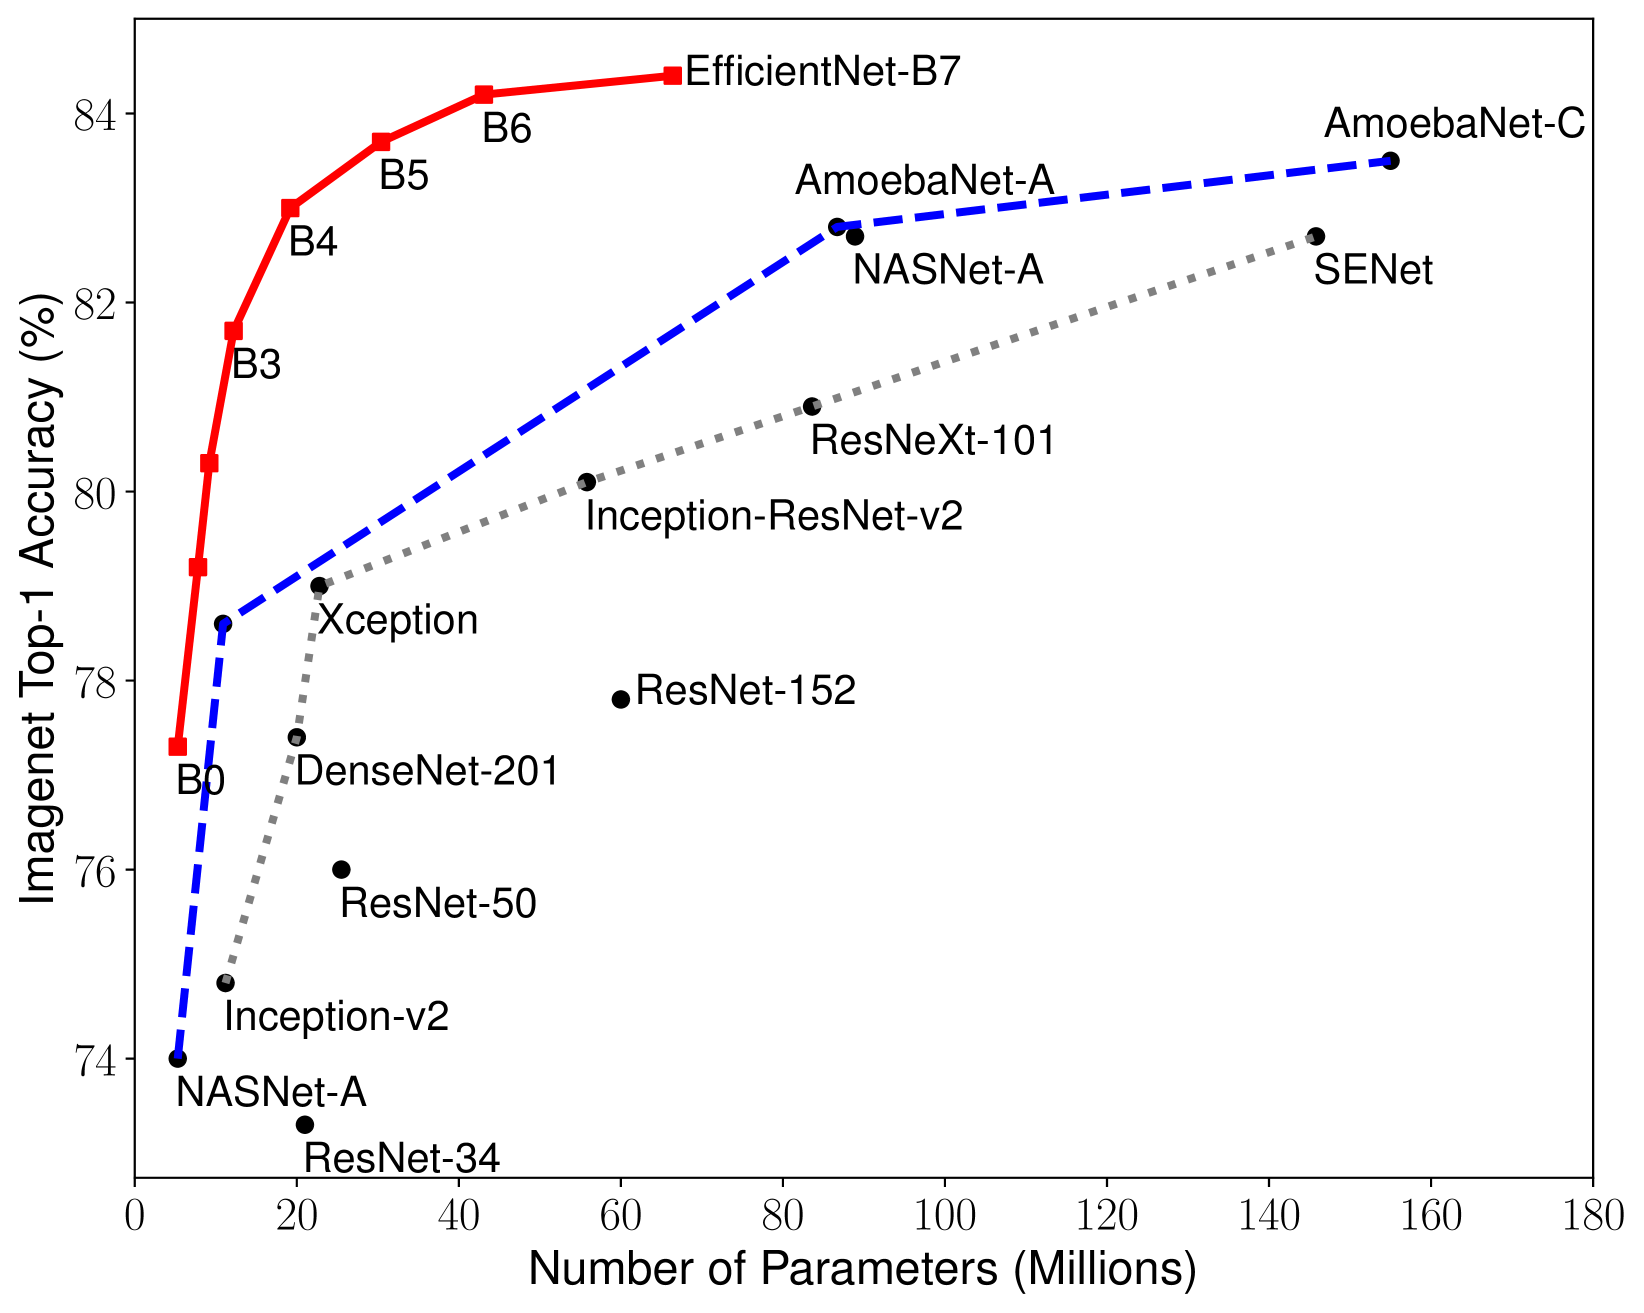
\includegraphics[width=0.45\textwidth]{./Graphics/efficientnet_performance.png}
   \caption{Estadísticas del rendimiento de los modelos de EfficientNet}
   \label{fig:efficientnet_performance}
   \end{center}
   \end{figure}

\subsection{EfficientNetB1}

En relación con el dataset HAM1000 \brackcite{ham10000}, la implementación del EfficientNetB1 puede ser particularmente beneficiosa para el análisis de datos. EfficientNetB1, entre las variantes de la serie EfficientNet, se encuentra en un punto medio en términos de complejidad y tamaño, ofreciendo un equilibrio entre precisión y eficiencia computacional. Dado que el HAM1000 es un conjunto de datos de imágenes dermatoscópicas que requiere una alta precisión en la identificación y clasificación de lesiones cutáneas, la utilización de EfficientNetB5 podría proporcionar una precisión y eficiencia aceptable en términos de recursos computacionales.

\subsection{Capas adicionales y regularización}

Para ajustar el modelo de EfficientNetB1 a nuestras necesidades, se añaden capas adicionales:

\begin{enumerate}
   \item Normalización por lotes: Esta capa busca estandarizar las activaciones del modelo para cada lote de entrenamiento. 
   La misma regulariza el modelo y, al mismo tiempo, suele acelera el entrenamiento ya que permite utilizar tasas de aprendizaje más altas. [\brackcite{regularization}]

   \item Densa: Se introduce una capa completamente conectada con 256 neuronas. Esta capa tiene una activación ReLU y utiliza regularización L1 y L2.
   La regularización L1 y L2 penaliza los pesos grandes en la red, ayudando a evitar el sobre-ajuste y garantizando que el modelo se generalice
    bien a nuevos datos. \brackcite{dense}
   
   \item Dropout: Esta técnica de regularización desactiva aleatoriamente una fracción (en este caso, el 45\%) de las neuronas durante el 
   entrenamiento. Esta aleatoriedad ayuda a evitar la dependencia excesiva en cualquier neurona individual, lo que a su vez ayuda a prevenir
    el sobre-ajuste. \brackcite{dropout}
   
   \item Capa de salida: Finalmente, se agrega una capa densa que tiene un número de neuronas igual al número de clases en nuestro problema. 
   La activación \textit{softmax} se utiliza aquí para transformar las salidas en probabilidades de clase.

\end{enumerate}

\subsection{Optimización}

Para el proceso de entrenamiento, se utiliza el optimizador \textit{Adamax} \brackcite{adamax}. Este es una variante del conocido optimizador Adam, que combina las ventajas de los métodos adaptativos de tasa de aprendizaje con una implementación más robusta en presencia de momentos espurios. 

Se configura el modelo para minimizar la categorical crossentropy, que es una medida común de error para problemas de clasificación, y se rastrea la precisión como métrica principal.

\subsection{Ajuste dinámico de la tasa de aprendizaje}

Una de las características más innovadoras de este enfoque es la inclusión de un "Callback" personalizado para ajustar dinámicamente la tasa de aprendizaje durante el entrenamiento. Este ajuste se basa en la precisión del entrenamiento y la pérdida de validación. En resumen, si el modelo no mejora lo suficientemente rápido (según ciertos criterios preestablecidos), la tasa de aprendizaje se reduce, con la esperanza de mejorar la convergencia del modelo \brackcite{lr}.

Este enfoque puede ser especialmente útil cuando nos enfrentamos a superficies de pérdida complejas con múltiples mínimos locales; al variar la tasa de aprendizaje, es más probable que el modelo salga de mínimos locales subóptimos y encuentre una solución mejor.

%-----------------------------------------------------------------------------------
\section{Resultados}\label{sec:results}
%-----------------------------------------------------------------------------------
En esta sección crucial de nuestra investigación, presentamos los resultados obtenidos a través de una serie de experimentos meticulosamente diseñados y ejecutados. Nuestro enfoque se centró en la exploración y optimización de diversos pipelines de procesamiento y clasificación de imágenes, cada uno configurado para evaluar distintos aspectos y técnicas dentro del amplio espectro del aprendizaje profundo y el análisis de imágenes.

Los experimentos se estructuraron con el objetivo de desentrañar las capacidades y limitaciones de varios modelos y técnicas en el contexto del procesamiento de imágenes. Cada experimento se diseñó con una configuración única, variando desde la selección de parámetros, la arquitectura de los modelos de aprendizaje profundo, hasta la técnica de preprocesamiento y aumento de datos. Este enfoque nos permitió observar los efectos específicos de cada variable en la precisión, eficiencia y efectividad de la clasificación.

Tras la implementación del modelo, los resultados obtenidos de este modelo de aprendizaje automático son muy útiles y eficientes en el campo de la detección de melanomas. Con una eficacia de validación cercana al 78,9\%, el modelo es capaz de detectar la presencia de melanoma con una precisión razonable. Los resultados son un paso significativo hacia la automatización del diagnóstico del cáncer de piel, que tradicionalmente ha dependido de la inspección visual por parte de expertos humanos.

La eficacia del modelo también puede mejorarse aún más optimizando su consumo de tiempo y memoria. Esta optimización será esencial para convertir los resultados del modelo en una solución a gran escala que pueda ser utilizada por profesionales sanitarios y pacientes de todo el mundo. Es importante señalar que el entrenamiento inicial del modelo es un proceso que se realiza una sola vez y no necesita ejecutarse continuamente. Por lo tanto, si se optimiza el proceso de entrenamiento, la eficacia del modelo puede mejorar considerablemente.

%-----------------------------------------------------------------------------------
	\subsection{Estadísticas básicas}\label{sub:basic_statistics}
%-----------------------------------------------------------------------------------
    
    Estos resultados de la tabla siguiente corresponden a la evaluación del modelo a lo largo de 40 epochs (o iteraciones) de entrenamiento. Cada fila representa una época y se presentan las siguientes métricas:
    
    \begin{description}
       \item [loss:] Es una medida de la diferencia entre las predicciones del modelo y los valores reales de los datos de entrenamiento en esa época. El objetivo del entrenamiento es minimizar esta métrica.
       \item [acc (accuracy):] Es la proporción de predicciones correctas realizadas por el modelo sobre el conjunto de datos de entrenamiento en esa época.
       \item [v loss (vl) (pérdida de validación):] Es la pérdida en el conjunto de datos de validación, que es un conjunto de datos independiente que no se utiliza para entrenar el modelo, sino para evaluar su generalizabilidad.
       \item [v acc (precisión de validación):] Es la precisión en el conjunto de datos de validación.
    \end{description}
\begin{figure}[ht]
        \small
        \begin{center}
            \begin{tabular}{|c|c|c|c|c|c|c|c|} \hline
            E  & Loss  & Acc & V loss & V acc & LR             & M & Batch \\ \hline
            1  & 9.535 & 37.735   & 9.396  & 38.4  & $10^{-2}$ & Acc     & 1337.97 \\ \hline
            2  & 7.791 & 66.306   & 7.832  & 61.6  & $10^{-2}$ & Acc     & 414.44 \\ \hline
            3  & 6.852 & 79.624   & 7.042  & 66.8  & $10^{-2}$ & Acc     & 291.03 \\ \hline
            4  & 6.191 & 85.544   & 6.398  & 67.6  & $10^{-2}$ & Acc     & 281.46 \\ \hline
            5  & 5.594 & 90.894   & 5.772  & 72.8  & $10^{-2}$ & Acc     & 288.00 \\ \hline
            6  & 5.111 & 92.943   & 5.311  & 74.4  & $10^{-2}$ & Vl  & 280.35 \\ \hline
            7  & 4.653 & 95.788   & 4.916  & 74.4  & $10^{-2}$ & Vl  & 274.80 \\ \hline
            8  & 4.268 & 95.788   & 4.631  & 73.6  & $10^{-2}$ & Vl  & 280.88 \\ \hline
            9  & 3.888 & 97.097   & 4.164  & 76.8  & $10^{-2}$ & Vl  & 302.48 \\ \hline
            10 & 3.547 & 97.553   & 3.840  & 76.4  & $10^{-2}$ & Vl  & 275.76 \\ \hline
            11 & 3.233 & 98.349   & 3.622  & 75.2  & $10^{-2}$ & Vl  & 281.52 \\ \hline
            \dots   & \dots   & \dots      & \dots    & \dots   & \dots    & \dots     & \dots \\ \hline
            31 & 0.592 & 99.488   & 1.133  & 77.2  & .00025 & Vl  & 420.26 \\ \hline
            \end{tabular}
            \caption{Estadísticas básicas de algunas iteraciones del modelo.}
        \end{center}\label{fig:modelo}
    \end{figure}
    
    En general, los resultados muestran que el modelo mejora con el tiempo, ya que la pérdida disminuye y la precisión aumenta tanto en el conjunto de datos de entrenamiento como en el de validación.

%-----------------------------------------------------------------------------------
	\subsection{Estadísticas de eficacia}\label{sub:accuracy_statistic}
%-----------------------------------------------------------------------------------
    La matriz de confusión proporciona información valiosa sobre el rendimiento del modelo en relacion de Actual/Predicho, en términos de su capacidad para clasificar correctamente cada una de las siete clases de cáncer de piel. 
    La diagonal principal de la matriz representa los verdaderos positivos (TP), el número de casos en los que el modelo ha predicho correctamente la clase correspondiente. Los valores fuera de la diagonal principal indican errores de clasificación. 
    Estos errores pueden ser falsos positivos (FP), falsos negativos (FN) o verdaderos negativos (TN), dependiendo de la posición en la matriz. 
    AKIEC, BCC, BKL, DF, MEL, NV y VASC son los acrónimos de los distintos tipos de lesiones cutáneas utilizados en la tarea de clasificación multiclase.

    Algunos patrones que pueden observarse en esta matriz son:

    \begin{enumerate}
       \item[.] El modelo parece tener dificultades para clasificar las muestras de la clase AKIEC, ya que sólo predice correctamente 5 de 7 casos. 
       Además, en la fila AKIEC hay un falso positivo (el modelo predijo la clase BKL en un caso que en realidad era AKIEC) y un falso negativo (el modelo predijo la clase MEL en un caso que en realidad era AKIEC). 
       \item[.] En la clase BCC, el modelo predice correctamente todos los casos.
       \item[.] Las muestras de las clases BKL y MEL parecen ser las más difíciles de clasificar, ya que hay varios falsos positivos y falsos negativos en esos rangos.
       \item[.] La mayoría de las predicciones se clasifican correctamente como NV, que es la clase más común en los datos.
    \end{enumerate}
    
    \begin{figure}[ht]%
		\begin{center}
		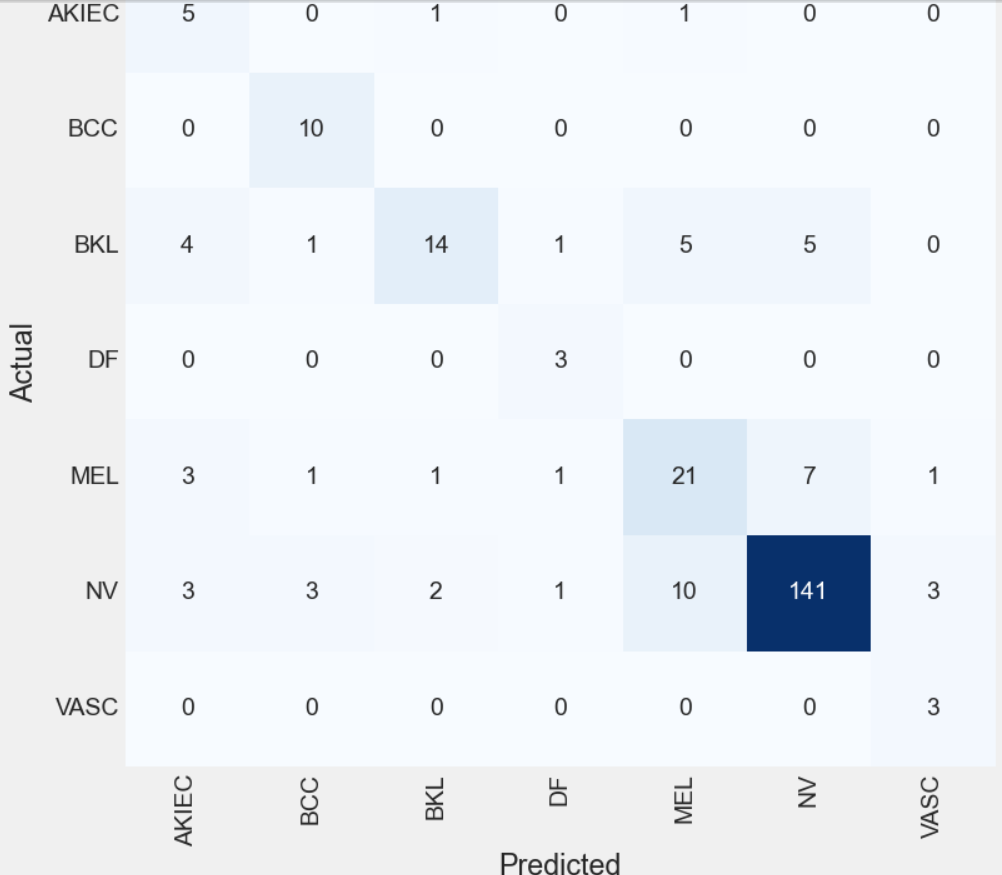
\includegraphics[width=0.45\textwidth]{./Graphics/confussion_matrix.png}
		\caption{Estadísticas de eficacia del modelo al estimar los resultados en el conjunto de pruebas.\label{fig:confussion_matrix}}
		\end{center}
		\end{figure}
    
    

%-----------------------------------------------------------------------------------
	\subsection{Estadísticas de aprendizaje}\label{sub:learning_statistics}
%-----------------------------------------------------------------------------------
		\begin{figure}[ht]%
      \begin{center}
      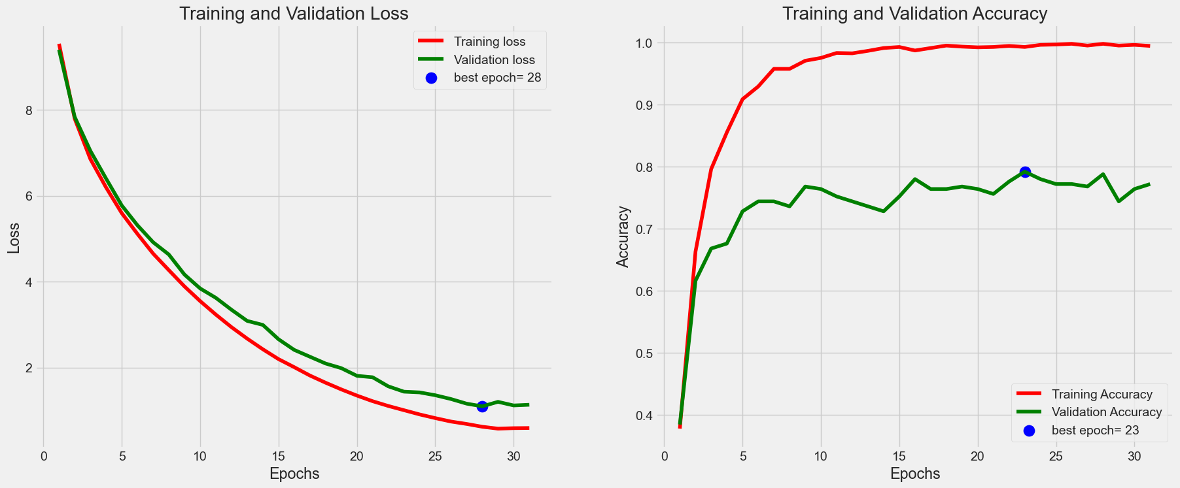
\includegraphics[width=0.45\textwidth]{./Graphics/training_validation.png}
      \caption{Estadísticas de aprendizaje a lo largo del proceso de entrenamiento (en rojo el proceso de entrenamiento en el conjunto de entrenamiento, en verde en el conjunto de validación).\label{fig:training_validation_loss}}
      \end{center}
		\end{figure}
  
La imagen anterior muestra un gráfico del curso temporal de las épocas realizadas, mostrando cómo el algoritmo iba obteniendo resultados más precisos y disminuyendo el error.

%-----------------------------------------------------------------------------------
\section{Ventajas y Desventajas}\label{sec:advantages_disadvantages}
%-----------------------------------------------------------------------------------
Las ventajas y desventajas del proceso son las siguientes. 
Ventajas: 
\begin{enumerate}
   \item Selección y representación del problema y de los datos. 
   Este proceso ayuda a comprender mejor el problema en cuestión y a identificar los datos relevantes necesarios para entrenar el modelo.
   \item Preprocesamiento de datos e imágenes. 
   Eliminar el ruido y los artefactos de las imágenes mejora la calidad de los datos y puede mejorar el rendimiento del modelo. 
   La selección de canales adecuados y la reducción del ruido también pueden mejorar el rendimiento del modelo
\end{enumerate}  
Desventajas: 	
\begin{enumerate}
   \item Modificación y procesamiento de datos. Si se utilizan conjuntos de datos inadecuados o se normalizan incorrectamente, el modelo puede no ser preciso o útil.
\end{enumerate} 

